\subsection{Monitoraggio e Intervento}
Il sistema di controllo e intervento scelto segue l'idea del controllo autonomo tramite l'utilizzo di 
una Neural ODE. Questo approccio permette di specificare un sistema di ODE che descrive il sistema reale 
con le sue relazioni e inserire chirurgicamente una rete neurale al suo interno che controlli il 
dosaggio delle contromisure. \cite{B_ttcher_2022} \cite{innes2019differentiable} \cite{sandoval2022neural}

Questa tecnica permette di ottenere ottimi risultati, i quali tuttavia dipendono fortemente dalla 
tipologia di modellazione del sistema scelto e dalla tipologia di funzione di costo o di controllo 
applicata per addestrare il modello. La sfida in questo caso ricade sull'attenta modellazione del 
sistema di partenza e sulla comprensione dei risultati offerti dal controllore. Questo controllore 
difatti ritorna dei valori nell'ambito $\in[0, 1]$, i quali possono essere difficilmente interpretabili.
Perciò è necessario a priori avere ben chiaro cosa significhi il range di valori che può ritornare
il controllore, e capire a cosa è associato nel mondo reale. 

Inizialmente la funzione di controllo inserita all'interno del modello ad agente è definita 
come riportato in figura \ref{fig:controller_abm}. è possibile osservare come vengano inseriti dei valori di 
controllo per gestire la chiamata al controllore vero e proprio.

I valori di controllo sono generalmente associati a quado bisogna realisticamente parlando, chiamare la 
funzione di controllo. Da un lato servono sia a ridurre il numero di chiamate, e quindi ridurre l'impatto 
prestazionale sia a rendere più realistica l'idea di avere accesso ad un sistema di controllo solamente 
in determinati punti del tempo e non sempre. Questo va ad imitare anche il ritardo tra la raccolta dati, 
la formulazione di una contromisura adeguata e l'applicazione della stessa.

Successivamente vengono definite ulteriori regole di attivazione, questa volta legate alla prima attivazione
del controllore. A posteriori è chiaro come avere delle regole di prevenzione già in atto possa essere di 
enorme aiuto nel combattimento contro il dilagare di un epidemia, ma alle volte vi è un ritardo nel riconoscere
il pericolo, e questo è dato dal valore di \emph{tolerance} il quale non attiva il controllore fintanto che 
la situazione sembra rimanere sotto i minimi di soglia. 

\begin{minipage}{\linewidth}
	\centering
	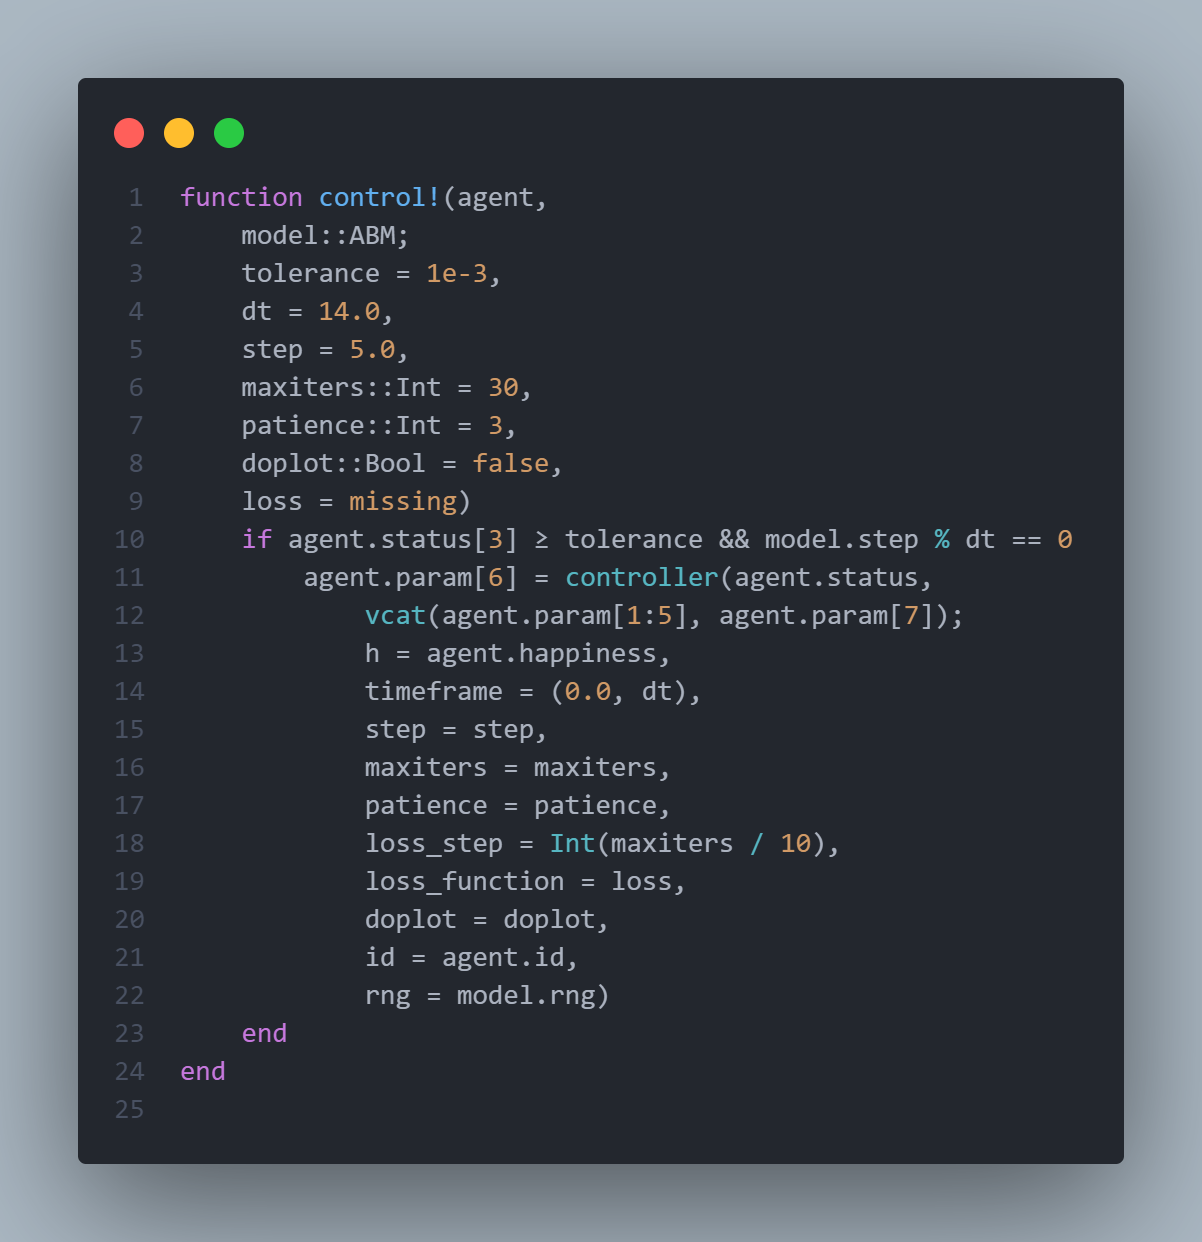
\includegraphics[width=\textwidth]{img/controller_neuralode.png}
	\captionof{figure}{Definizione controller all'interno del modello ad agente}
	\label{fig:controller_abm}
\end{minipage}

Altri valori definiscono principalmente i parametri che servono alla funzione di controllo per operare correttamente.
Tra questi vi è un parametro opzionale $\upsilon$ il quale descrive quanto potrà essere il valore massimo delle 
contromisure applicabili in relazione a quanti infetti sono presenti all'interno di un dato nodo. Questo valore viene 
calcolato come un esponenziale nel numero degli infetti. Questa assunzione è utile come valore di appoggio ulteriore 
per il controllore nel caso in cui dovesse ritornare un valore troppo alto rispetto a quello che di buon senso sarebbe 
adatto. 

\begin{minipage}{\linewidth}
	\centering
	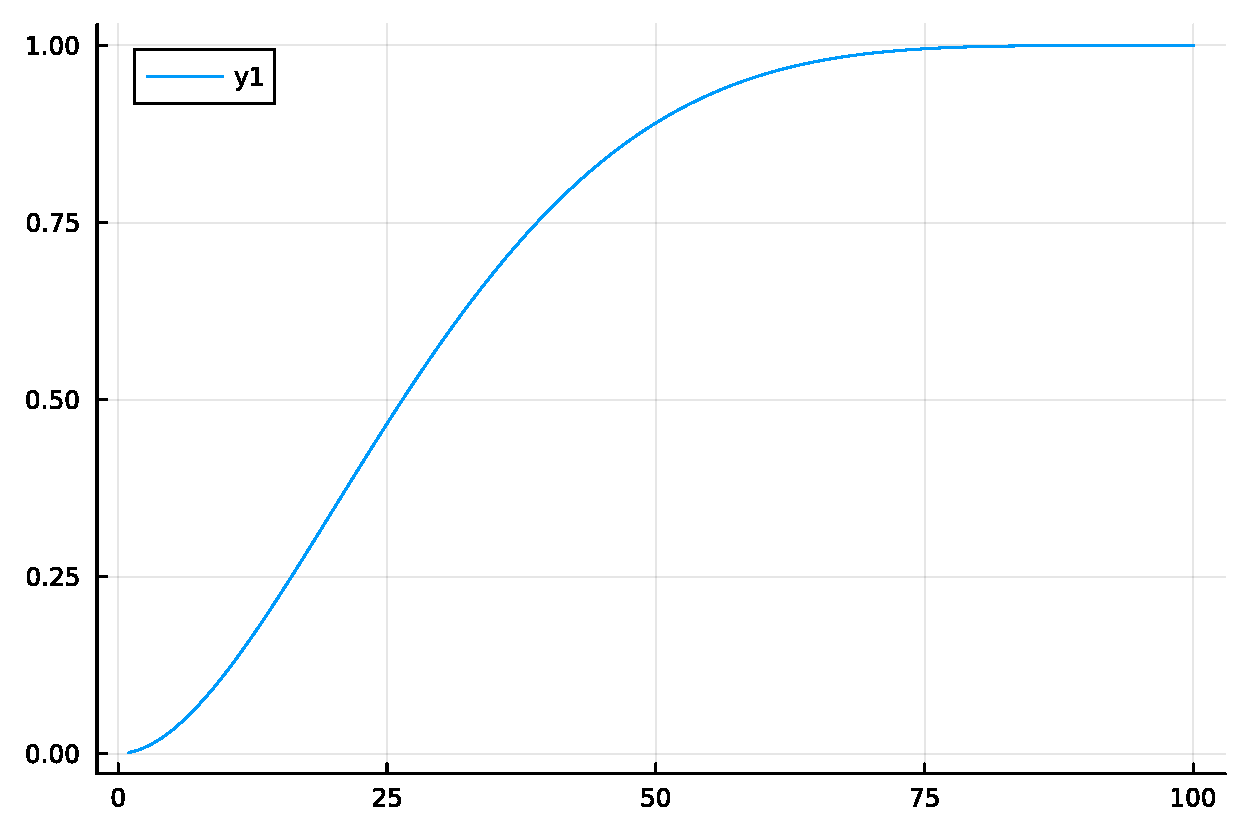
\includegraphics[width=\textwidth]{img/beta_cdf.pdf}
	\captionof{figure}{Funzione per il calcolo del limite superiore per le contromisure non farmaceutiche}
	\label{fig:max_countermeasures_function_abm}
\end{minipage}

Come si può osservare, la funzione descritta in figura \ref{fig:max_countermeasures_function_abm} 
descrive la \emph{funzione di distribuzione cumulativa} per la distribuzione \emph{beta} \cite{wiki:Beta_distribution} 
con parametri $\alpha = 2$ e $\beta = 5$. Questo tipo di funzione è stata scelta in quanto descrive abbastanza 
bene il valore di pericolo che, soprattutto durante i primi mesi di pandemia, è stato attribuito al numero di infetti che 
si riscontravano. Questo valore cresce rapidamente e poi tende a rallentare abbastanza bruscamente una volta superata la 
soglia del cinquanta percento di infetti. 

Questo può essere anche relazionato all'idea che una pandemia abbia un punto critico dopo il quale le speranze decadono. Questo 
ovviamente in relazione alla pandemia stessa. Questa funzione potrebbe anche alterarsi nel corso del tempo, modellando perciò 
una sorta di abitudine alla pandemia. 

Il controllore vero e proprio si articola principalmente come già accennatto nella sezione relativa alle Neural ODE. 

\begin{minipage}{\linewidth}
	\centering
	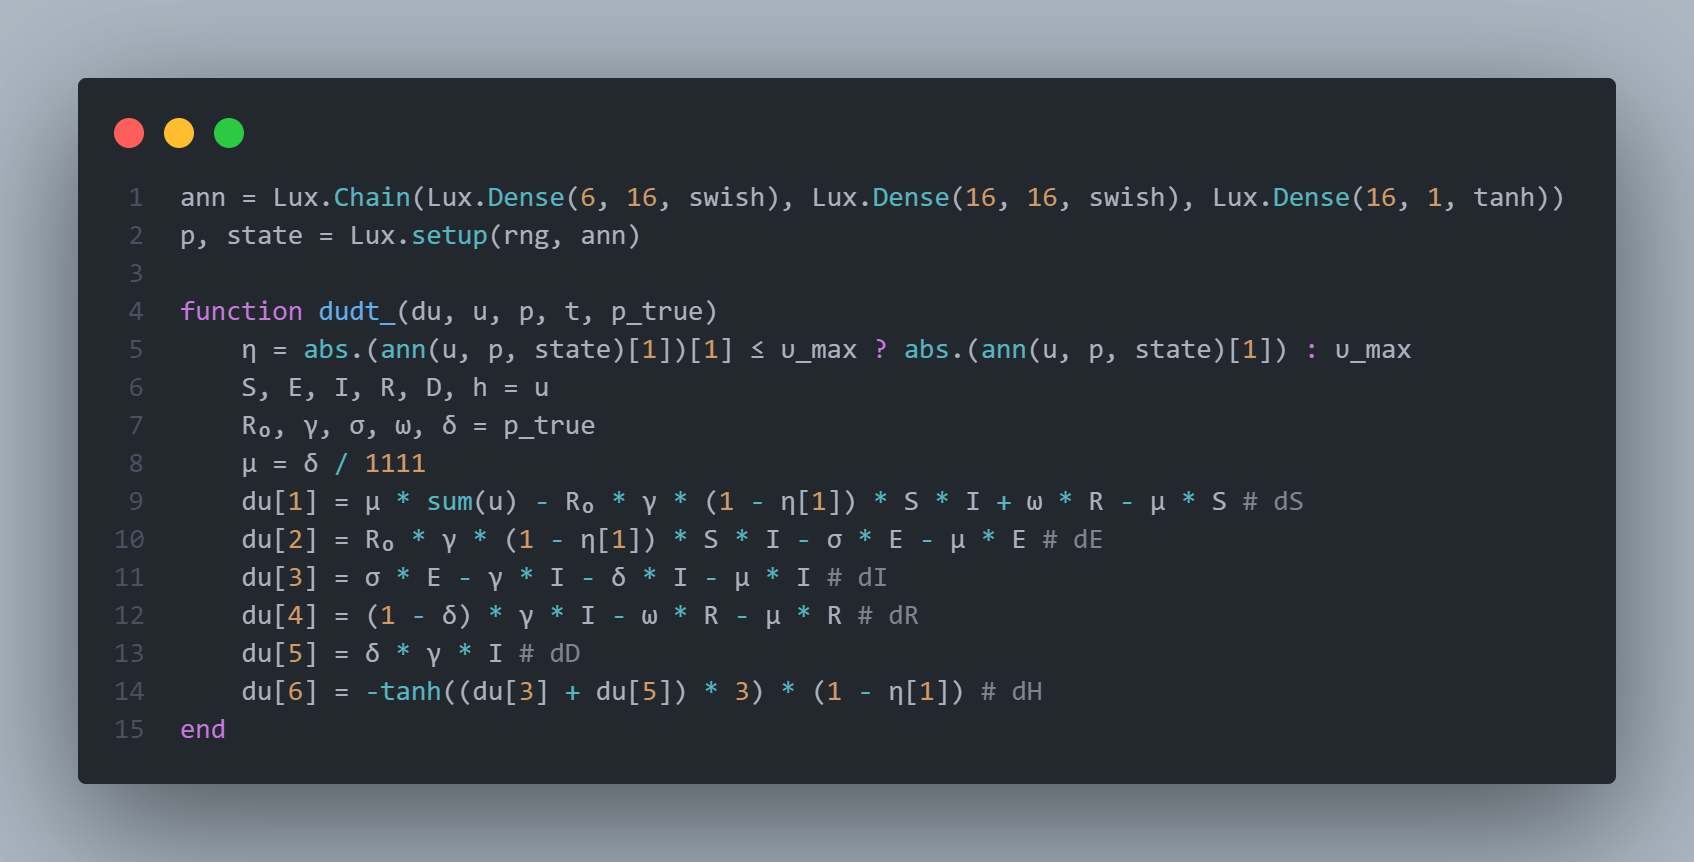
\includegraphics[width=\textwidth]{img/controller1.png}
	\captionof{figure}{Definizione controllore tramite Neural ODE}
	\label{fig:controller1}
\end{minipage}

Viene definita una rete neurale tramite l'ausilio del framework \textbf{Lux.jl} \cite{pal2023lux}, e questa viene utilizzata
esclusivamente per il guess del valore di controllo $\eta$ durante la fase di addestramento, il quale verrà 
alla fine utilizzato come valore di controllo per il modello. Successivamente viene definito il sistema di ODE che governa il fenomeno che vogliamo analizzare, nello specifico il sistema in 
questione è un sistema \textbf{SEIR} che modella la perdita di immunità con il tempo. 

Successivamente viene istanziato il problema con l'ausilio dell'interfaccia \textbf{ODEProblem} e da qui in avanti il modello potrà iniziare a 
essere allenato. Innanzitutto vengono definite delle funzioni per la predizione e il calcolo della loss del modello, 
e infine anche una funzione ausiliaria di callback utile per osservare l'andamento dell'apprendimento del modello.

\begin{minipage}{\linewidth}
	\centering
	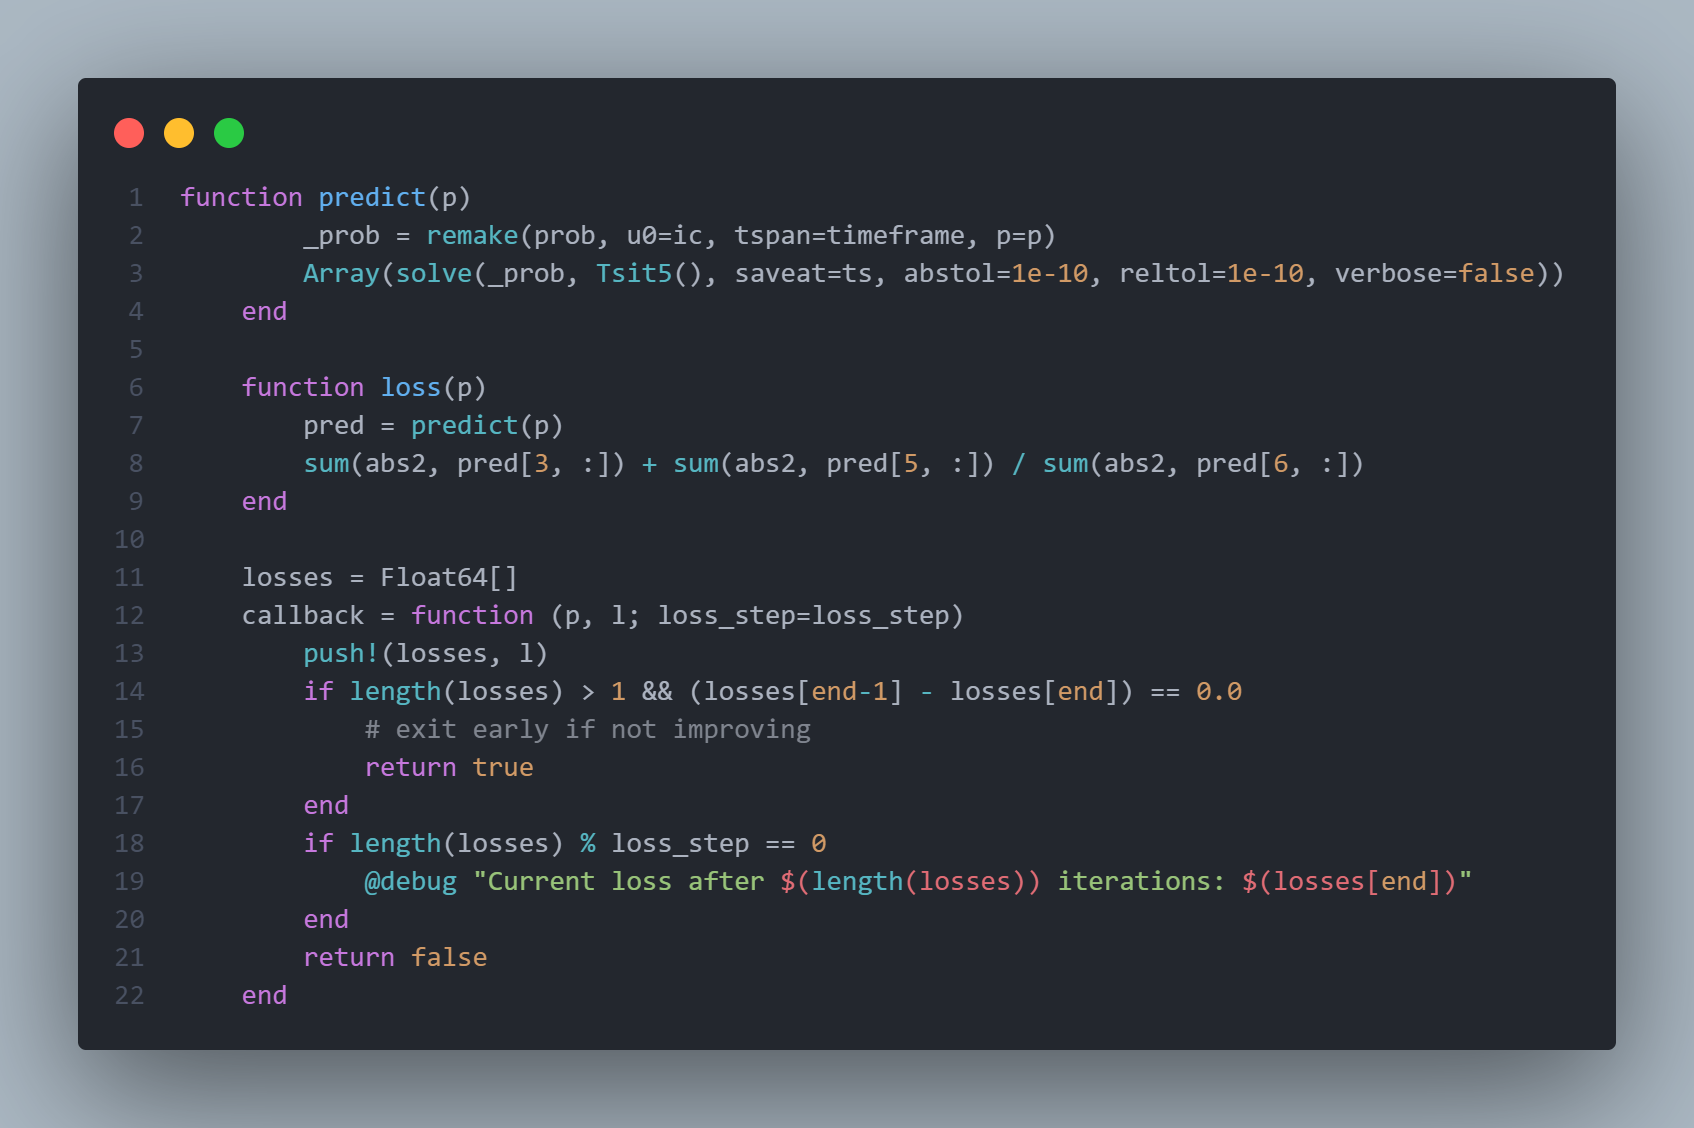
\includegraphics[width=\textwidth]{img/controller2.png}
	\captionof{figure}{Definizione funzioni di appoggio del controllore}
	\label{fig:controller2}
\end{minipage}

Come si può osservare in figura \ref{fig:controller2} la funzione di \emph{callback} oltre ad essere una funzione di 
appoggio nella stampa dei dati relativi all'addestramento, è anche una utile funzione per implementare un controllo sulla tipologia 
di apprendimento del modello. Infatti per ridurre ancora di più il numero di iterazioni necessarie per avere dei buoni risultati 
è stato scelto di inserire un controllo simile al metodo di \textbf{early stopping} \cite{wiki:Early_stopping} per prevenire 
l'addestramento eccessivo quando si trova un valore di ottimo. Questo approccio è puramente \emph{empirico} in quanto 
è stato riscontrato come il valore di loss generale del sistema tende a decrescere o crescere stabilmente e una volta trovato il 
valore ottimale, se rimangono delle iterazioni da fare, questo non migliora per cui una volta che i valori rimangono identici 
è un buon azzardo terminare il periodo di addestramento del modello.

La parte di addestramento vero e proprio del modello avviene con le seguenti funzioni

\begin{minipage}{\linewidth}
	\centering
	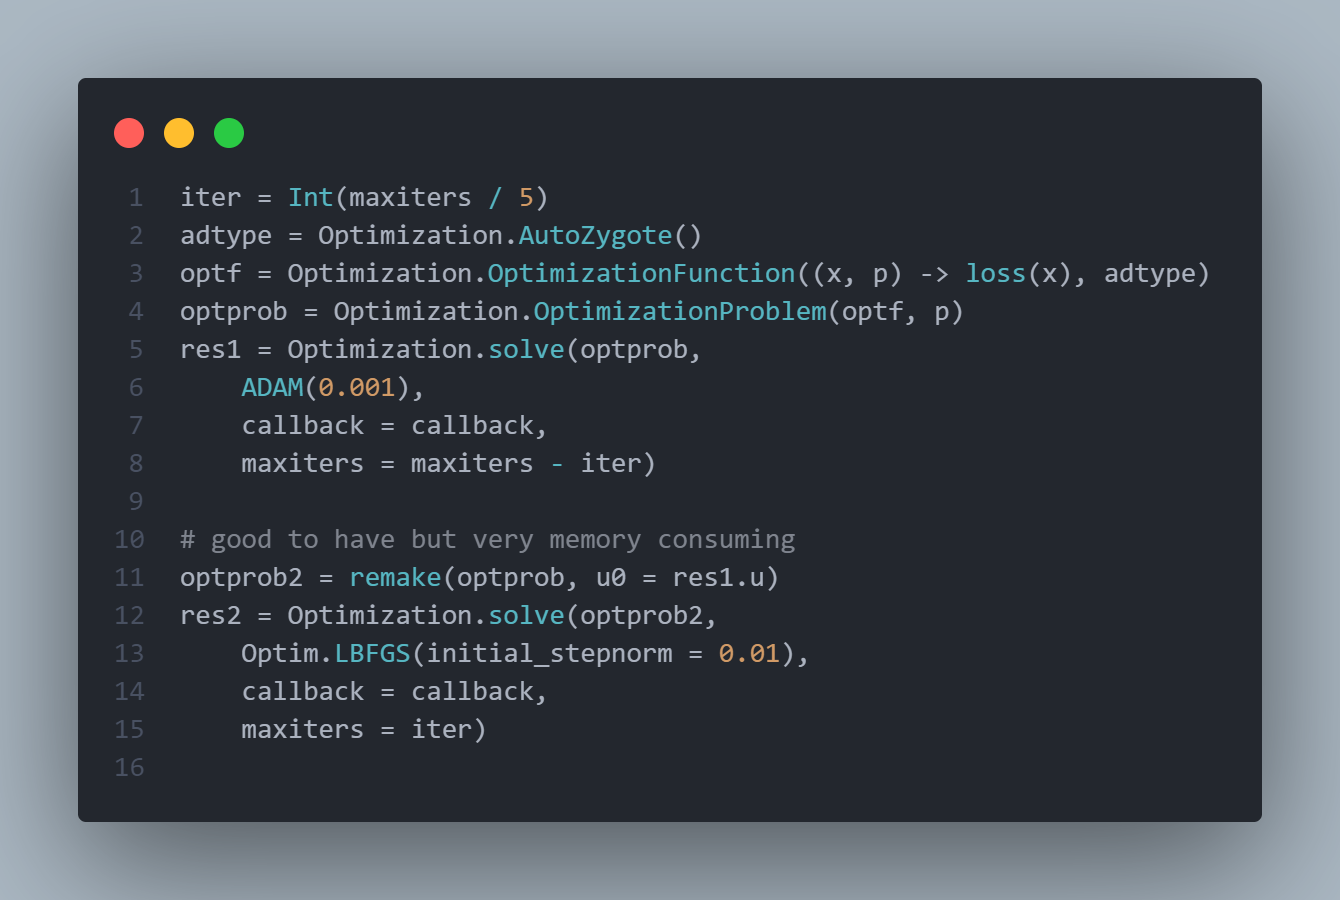
\includegraphics[width=\textwidth]{img/controller3.png}
	\captionof{figure}{Definizione funzioni di addestramento del controllore}
	\label{fig:controller3}
\end{minipage}

Il ciclo di addestramento può essere scomposto idealmente in due parti, ma per quanto osservato, non sono 
entrambe necessarie. La prima parte, riportata in figura \ref{fig:controller3} si propone di utilizzare un ciclo di addestramento 
con l'utilizzo dell'ottimizzatore \textbf{ADAM}. Se i risultati dovessero esser soddisfacenti, allora è possibile terminare. 
Tuttavia in questi casi, è buona pratica utilizzare due differenti cicli di addestramento per migliorare i risultati. 

Più nello specifico vengono associati due differenti cicli di addestramento con due differenti ottimizzatori per ottenere il massimo 
da entrambi. Questo approccio serve per massimizzare le peculiarità di ognuno degli ottimizzatori. è pratica comune utilizzare per la 
buona parte dell'addestramento un ottimizzatore in grado di trovare un buono spazio degli iperparametri e successivamente utilizzare 
un ottimizzatore come ad esempio \textbf{BFGS} \cite{10.1093/imamat/6.1.76} \cite{35d0019d-775a-3628-b0b4-67be112e346b} \cite{10.1093/comjnl/13.3.317} \cite{e3177091-3094-3792-9d61-0ab445735ddb}
il quale è estremamente utile nel trovare rapidamente un minimo locale all'interno dello spazio dei parametri.

L'utilizzo di questi due ottimizzatori in successione è utile in quanto utilizzando solamente \textbf{ADAM} si potrebbe 
incorrere nell'avere un numero di iterazioni troppo elevate per raggiungere lo stesso risultato, mentre utilizzando solamente \textbf{BFGS} si 
potrebbe incorrere in un brutto minimo locale.

La mia scelta di non utilizzare l'approccio sopra descritto, ovvero di utilizzare due differenti ottimizzatori per 
ottenere il massimo risultato da entrambi, è dato dal fatto che generalmente l'utilizzo di ADAM 
con un numero di iterazioni molto contenuto, dato anche dall'utilizzo di una tecnica per ridurre ulteriormente
le iterazioni di addestramento se non vi è un guadagno di accuratezza \ref{fig:controller2}, 
permette di arrivare al miglior risultato in breve tempo senza l'utilizzo di un 
secondo ottimizzatore, il quale se comunque utilizzato non porta alcun 
miglioramento di sorta, impegnando solamente risorse computazionali.

\begin{minipage}{\linewidth}
	\centering
	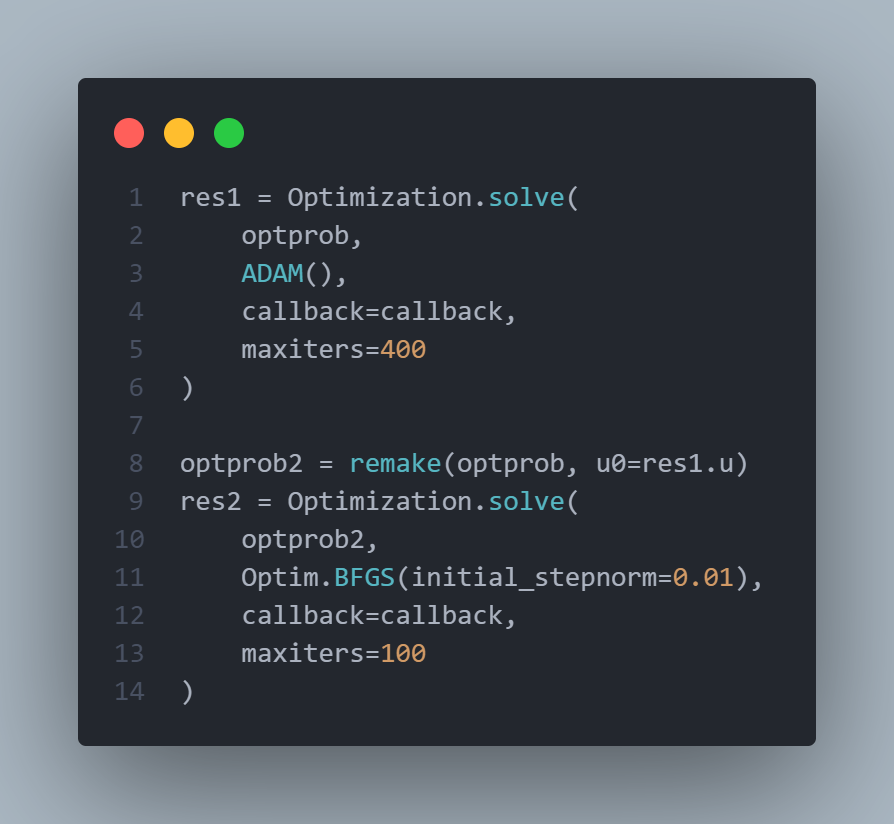
\includegraphics[width=\textwidth]{img/optimizers_example.png}
	\captionof{figure}{Esempio di utilizzo congiunto di due ottimizzatori differenti in uno stesso ciclo di addestramento}
	\label{fig:two_otpimizers}
\end{minipage}

\subsubsection*{Funzione di attivazione rete neurale}
% inserisci qualcosa in più
La scelta della funzione di attivazione all'interno delle reti neurali pone un grande impatto sulle 
dinamiche di apprendimento. Attualmente la più utilizzata e di grande successo è la \textbf{ReLU}
(\textbf{Re}ctified \textbf{L}inear \textbf{U}nit) la quale è della forma $f(x) = max(0,x)$. 
Tuttavia svariate alternative sono state proposte, ma nessuna di queste è riuscita a 
spodestare il primato della ReLU, principalmente a causa di guadagni prestazionali inconsistenti. 

La funzione di attivazione che ho deciso di utilizzare si chiama \textbf{Swish} ed è stata proposta dal 
\emph{Google Brain Team} \cite{ramachandran2017searching}, la quale è la seguente funzione $f(x) = x \cdot sigmoid(x)$. 
Nei loro esperimenti è stato osservato come sostituire la funzione di attivazione ReLU con Swish permetteva 
di avere un aumento prestazionale sui task di \emph{top-1 classification} sul dataset \textbf{ImageNet} del $0.9\%$ utilizzando
\textbf{NASNetA} e dello $0.6\%$ utilizzado \textbf{Inception-ResNet-v2}. 

\begin{minipage}{\linewidth}
	\centering
	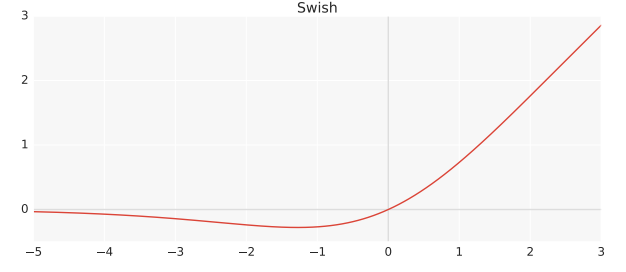
\includegraphics[width=\textwidth]{img/Screen-Shot-2017-10-18-at-2.39.55-PM.png}
	\captionof{figure}{Funzione di attivazione Swish}
	\label{fig:swish}
\end{minipage}

Il punto forte di Swish è la sua semplicità e forte somiglianza con ReLU, la quale la rende estremamente facile da implementare
al suo posto. La principale problematica con l'utilizzo di ReLU è il fatto che il valore della derivata è 0 per metà 
dei valori in input $x$. 

è stato dimostrato come, utilizzando il dataset \textbf{MNIST}, le prestazioni di Swish e ReLU siano 
equiparabili nei fintanto che le reti avevano un numero di layer all'incirca fino a 40. Successivamente Swish riusciva ad ottenere 
prestazioni migliori di ReLU in maniera considerevole, soprattutto quando il numero di layer si attestava tra i 40 e i 50, casi 
in cui l'ottimizzazione tendenzialmente diventa più complessa. Questo suggeri, e venne poi osservato, come 
in reti molto profonde, Swish tendeva ad avere prestazioni migliori nei test di accuracy rispetto alla controparte presa in esame. 
Entrambe comunque hanno esperienziato un calo delle prestazioni all'aumentare della dimensioni dei batch; in ogni caso comunque Swish otteneva 
dei risultati migliori. 

Alla luce di questi dati ho deciso di utilizzare questa funzione come funzione di attivazione all'interno della rete neurale, 
anche se tendenzialmente essendo essa poco profonda, i risultati e soprattutto il guadagno di accuratezza non dovrebbe essere troppo sensibile \ref{fig:controller1}.